\subsection{ClaraX: Verzerrungsreduziertes Crawling}

\begin{frame}
  {Problem: Breadth-First-Search-Crawling}
  \begin{itemize}
    \item Crawling: neue Webseiten auf Basis der Links\\
      in bereits bekannten Webseiten finden
    \item Queueing-Strategie bestimmt Crawling-Algorithmus
    \item typisches BFS: alle Links in Reihenfolge des Auffindens queuen
      \vspace{0.5cm}
    \item BFS: bekannter nicht-korrigierbare Verzerrung\\
      abhängig vom \alert{Eingangsgrad}
  \end{itemize}
\end{frame}

\begin{frame}
  {Ist Verzerrung ein Problem?}
  \begin{itemize}
    \item je nach Anwendungsszenario\ldots
    \item für theoretische linguistische Fragestellungen,\\
      wie sie uns interessieren: \alert{Ja!}
    \item auch ohne Glauben an Balanciertheit/Repräsentativität:\\
      starke unbekannte Verzerrung macht \alert{nie} gute Stichproben
    \item vgl.\ SECOW11: 75\% aller Dokumente vom selben Bloghoster
      \vspace{0.5cm}
    \item wenigstens: Effekte aus Korpuszusammensetzung untersuchen:\\
      DFG \textit{Webcharakterisierung} (SCHA1619-1)
  \end{itemize}
\end{frame}

\begin{frame}
  {Lösung: Korrigierte Random Walks}
  \begin{itemize}
    \item Random Walks: Verzerrung nach \alert{PageRank}
    \item wenn PageRank bekannt oder schätzbar,\\
      Verzerrungskorrektur durch Rejection Sampling möglich
    \item verschiedene Methoden, unterschiedlich impraktibabel
    \item auf jeden Fall: maximal kleine Referenzkorpora: \alert{RandyCOW}
  \end{itemize}
\end{frame}

\begin{frame}
  {ClaraX}
  \begin{itemize}
    \item voll bemerkmalter Random Walker
    \item Politeness: voll, reduziert, gar nicht, stealth mode(s)
    \item Dead-end-Strategien: terminate, jump, backtrack
    \item scope restriction\slash black \& white list
    \item follow modes: same host, same virtual host, different host oder Kombinationen
    \item Verarbeitung eingebaut: Spracherkennung, Dokumentqualität, Boilerplate, etc. (texrex)
    \item praktisch Möglich: Einschränkung auf\\
      bestimmte \alert{Segmente} des WWW
  \end{itemize}
\end{frame}

\begin{frame}
  {Baseline-Experiment 1: True Random Walking}
  \begin{itemize}
    \item jedem Link folgen (auch intern)
    \item nur deutsche Dokumente (step back wenn nicht Deutsch)\\
      in \textit{at}, \textit{ch}, \textit{de}
    \item 12.75 Tage, 1 Millionen Schritte
    \item entdeckte Hosts: \alert{1,227}
    \item durchschnittliche Verweildauer auf Host: \alert{16.42} Schritte
    \item mittlere Anzahl Dokumente pro Host: \alert{890.83}
  \end{itemize}
\end{frame}

\begin{frame}
  {Baseline-Experiment 2: Host Walking}
  \begin{itemize}
    \item Ineffizienz von seitenweisem Random Walk: \alert{Host Walk}
    \item follow mode: different (virtual) host
    \item 25.36 Tage, 2.090.443 Schritte
    \item mittlere Anzahl Dokumente pro Host: \alert{10.25} (statt 890.83)
    \item Problem: aggressives Rejection Sampling braucht\\
      noch längere Walks
  \end{itemize}
\end{frame}

\begin{frame}
  {Effekt von aggressivem Rejection Sampling}
  Relativ zu einer \alert{gewünschten} Korpusgröße:\\
  \vspace{0.5cm}
  \centering
  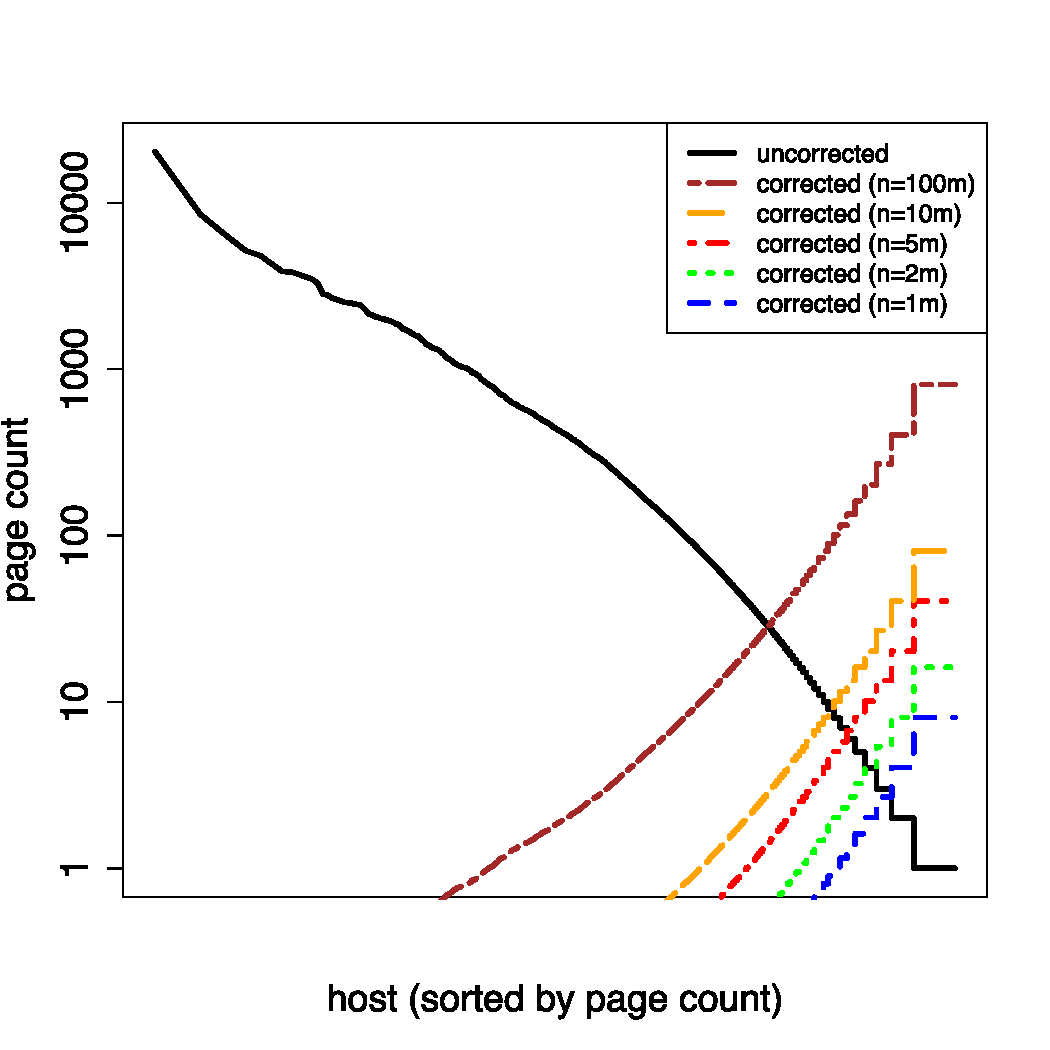
\includegraphics[width=0.5\textwidth]{graphics/corrected}\\
  \vspace{0.1cm}
  \pause
  \raggedright
  Was kann man da machen? \ldots
\end{frame}
